\documentclass[12pt]{article}

\usepackage[utf8]{inputenc}
\usepackage[english]{babel}
\usepackage{amssymb}
\usepackage{amsfonts}
\usepackage{setspace}
\usepackage{algorithm}
\usepackage[noend]{algpseudocode}
\usepackage{amsmath}
\usepackage{graphicx}
\usepackage[margin=1in]{geometry}
\usepackage[hidelinks]{hyperref}
\usepackage{float}
\usepackage[danish]{varioref}
\usepackage{multirow}
\usepackage{hhline}
\usepackage{inconsolata}
\usepackage{etoolbox}
\usepackage[usenames,dvipsnames]{xcolor}
\usepackage{tikz}
\usetikzlibrary{positioning,shapes, shadows, arrows}
\usepackage{listings}

%%%%%%%%%%%%%%%%%%%%%%%%%
%         Colors        %

\definecolor{dark-blue}{HTML}{000080}
\definecolor{dark-green}{HTML}{008000}
\definecolor{pale-purple}{HTML}{94558D}
\definecolor{dark-purple}{HTML}{0000AA}
\definecolor{regular-purple}{HTML}{660099}
\definecolor{magenta}{HTML}{B200B2}
\definecolor{light-gray}{HTML}{FAFAFA}
\definecolor{theorem-gray}{HTML}{F5F5F5}
\definecolor{dark-gray}{HTML}{2D2D2D}
\definecolor{comment}{HTML}{808080}
\definecolor{digit}{HTML}{0000FF}

%                       %
%%%%%%%%%%%%%%%%%%%%%%%%%

%%%%%%%%%%%%%%%%%%%%%%%%%
%        Theorem        %

\usepackage{amsthm}
\usepackage{thmtools}
\theoremstyle{definition}

\declaretheoremstyle[
spaceabove=6pt, spacebelow=6pt,
headfont=\normalfont\bfseries,
notefont=\mdseries, notebraces={(}{)},
bodyfont=\normalfont,
postheadspace=1em,
shaded={bgcolor=theorem-gray}
]{exstyle}

\declaretheoremstyle[
spaceabove=6pt, spacebelow=6pt,
headfont=\normalfont\bfseries,
notefont=\mdseries, notebraces={(}{)},
bodyfont=\normalfont,
postheadspace=1em,
shaded={bgcolor=theorem-gray}
]{defstyle}

%\declaretheorem[thmbox=M]{definition}
\declaretheorem[style=defstyle]{definition}
%\declaretheorem[thmbox=M]{example}
\declaretheorem[style=exstyle]{example}

%                       %
%%%%%%%%%%%%%%%%%%%%%%%%%

%%%%%%%%%%%%%%%%%%%%%%%%%
%   subsubsubsection    %

\usepackage{titlesec}
\titleclass{\subsubsubsection}{straight}[\subsection]

\newcounter{subsubsubsection}[subsubsection]
\renewcommand\thesubsubsubsection{\thesubsubsection.\arabic{subsubsubsection}}

\titleformat{\subsubsubsection}
  {\normalfont\normalsize\bfseries}{\thesubsubsubsection}{1em}{}
\titlespacing*{\subsubsubsection}
{0pt}{3.25ex plus 1ex minus .2ex}{1.5ex plus .2ex}

\makeatletter
\def\toclevel@subsubsubsection{4}
\def\l@subsubsubsection{\@dottedtocline{4}{7em}{4em}}
\makeatother

\setcounter{secnumdepth}{4}
\setcounter{tocdepth}{4}

%                       %
%%%%%%%%%%%%%%%%%%%%%%%%%

%%%%%%%%%%%%%%%%%%%%%%%%%
%          Tikz         %

\tikzset{
  treenode/.style = {align=center, inner sep=0pt, text centered,
    font=\sffamily},
  arn_n/.style = {treenode, circle, black, font=\sffamily\bfseries, draw=white, fill=white, text width=1.5em}
}

%                       %
%%%%%%%%%%%%%%%%%%%%%%%%%

%%%%%%%%%%%%%%%%%%%%%%%%%
%       Algorithm       %

\usepackage{xspace}
\usepackage{algpseudocode}
\newcommand*\Let[2]{\State #1 $\gets$ #2}
\newcommand*\Returns[1]{\State \Return #1}
\newcommand*\Append[2]{\State $#1 << #2$}
\algrenewcommand\algorithmicrequire{\textbf{Input:}}
\algrenewcommand\algorithmicensure{\textbf{Output:}}
\renewcommand{\algorithmicforall}{\textbf{foreach}}
\algnewcommand{\Or}{\textbf{or}\xspace}
\algnewcommand{\Not}{\textbf{not}\xspace}
\algnewcommand{\In}{\textbf{in}\xspace}

%                       %
%%%%%%%%%%%%%%%%%%%%%%%%%

\setlength\parindent{0pt}
\usepackage[parfill]{parskip}

\newcommand*{\FormatDigit}[1]{\textcolor{digit}{#1}}

\lstset{
	language=Ruby,
	prebreak=\raisebox{0ex}[0ex][0ex]{\ensuremath{\color{red}\space\hookleftarrow}},
	basicstyle=\footnotesize\ttfamily,
	%
	literate=%
    	{0}{{\FormatDigit{0}}}{1}%
        {1}{{\FormatDigit{1}}}{1}%
        {2}{{\FormatDigit{2}}}{1}%
        {3}{{\FormatDigit{3}}}{1}%
        {4}{{\FormatDigit{4}}}{1}%
        {5}{{\FormatDigit{5}}}{1}%
        {6}{{\FormatDigit{6}}}{1}%
        {7}{{\FormatDigit{7}}}{1}%
        {8}{{\FormatDigit{8}}}{1}%
        {9}{{\FormatDigit{9}}}{1}%
        {.0}{{\FormatDigit{.0}}}{2}% Following is to ensure that only periods
        {.1}{{\FormatDigit{.1}}}{2}% followed by a digit are changed.
        {.2}{{\FormatDigit{.2}}}{2}%
        {.3}{{\FormatDigit{.3}}}{2}%
        {.4}{{\FormatDigit{.4}}}{2}%
        {.5}{{\FormatDigit{.5}}}{2}%
        {.6}{{\FormatDigit{.6}}}{2}%
        {.7}{{\FormatDigit{.7}}}{2}%
        {.8}{{\FormatDigit{.8}}}{2}%
        {.9}{{\FormatDigit{.9}}}{2}%
        %{,}{{\FormatDigit{,}}{1}% depends if you want the "," in color
        {\ }{{ }}{1}% handle the space
		{æ}{{\ae}}1
        {ø}{{\o}}1
        {å}{{\aa}}1
        {Æ}{{\AE}}1	
        {Ø}{{\O}}1
        {Å}{{\AA}}1
        {~}{{$\scriptstyle{\sim}$}}1, % handle tilde ~
	%
	%emph={@param,@return},
	otherkeywords={},
	keywords=[2]{self},
	keywords=[3]{__init__},
	keywords=[4]{object},
	keywords=[5]{encoding, flags},
	keywords=[6]{map},
	%
	keywordstyle=\bfseries\color{dark-blue},
	keywordstyle={[2]\color{pale-purple}},
	keywordstyle={[3]\color{magenta}},
	keywordstyle={[4]\color{dark-blue}},
	keywordstyle={[5]\color{regular-purple}},
	keywordstyle={[6]\color{dark-purple}},
	keywordstyle={[7]\bfseries\color{black}},
    commentstyle=\itshape\color{comment},
    identifierstyle=\color{black},
	stringstyle=\bfseries\color{dark-green},
	%emphstyle=\bfseries,
	%
	numbers=left, % where to put the line-numbers
	numberstyle=\ttfamily\color{dark-gray},
	numbersep=5pt, % how far the line-numbers are from the code
	stepnumber=1,
	showstringspaces=false,
	backgroundcolor=\color{light-gray},
	tabsize=4,
	captionpos=b, % sets the caption-position to bottom
	breaklines=true % sets automatic line breaking
}

\linespread{1.3}

\begin{document}

\begin{titlepage}
    \vspace*{\fill}
    \begin{center}
      {\Huge Midtvejsrapport Bachelorproject}\\[0.7cm]
      {\Large Regular Expression Matching In Genomic Data}\\[0.4cm]
      {\large Rasmus Haarslev - nkh877}\\
      {\large Troels Thomsen - qvw203}\\[0.4cm]
      {\textbf{Supervisors:}\\
      Rasmus Fonseca\\
      Niels Bjørn Bugge Grathwohl\\
      Ulrik Rasmussen\\
      Martin Asser Hansen}\\
      {\small \textbf{April 30th 2015}}\\[0.3cm] 
      {\small Department of Computer Science}\\
      {\small University of Copenhagen}
    \end{center}
    \vspace*{\fill}
\end{titlepage}	

\clearpage
\pagenumbering{gobble}
\thispagestyle{empty}

\newpage

\tableofcontents
\newpage

\pagenumbering{arabic}

\section{Abstract (TO BE WRITTEN)}
\section{Introduction}

Institute for microbiology at University of Copenhagen has a large collection of sequenced DNA material stored on their servers. They estimate somewhere between two and three petabytes of data stored in FASTA and FASTQ files \textbf{NEED REF}.

Parsing and analysing this large amount of data poses several challenges. Searching through the files with simple text search is not advanced enough. DNA contains a lot of redundancy and variation over similar concepts, which means that two seemingly different sequences can have very similar functionality or interact with other components in a similar way. \\
This requires the search functionality to be able to allow for a great deal of variance and flexibility in the sequences which are searched for.

Currently, the state-of-the-art method for searching through genomic data is the scan-for-matches program developed by Ross Overbeek, David Joerg and Morgan Price\cite{scan-for-matches}, which is able to locate complex DNA patterns, such as looking for a random 8 character sequence, repeated 20 characters ahead, and in reverse. These patterns will be referred to as \textit{patscan patterns}, while the program itself will be referred to as \textit{scan-for-matches}.

While scan-for-matches performs very well and has a very compact language, it is not very user friendly \textbf{NEED REF} and have some unfortunate limitations when running many consecutive scans.

Recently, the KMC group have developed a regular expression implementation, which we will refer to as the KMC engine, which so far has shown competitive performance, compared to current industry standard engines\cite{two-pass-greedy}.
We are hoping that optimized regular expressions running on the KMC engine will be able to match or outperform scan-for-matches.
If we could achieve a performance improvement over scan-for-matches, it would greatly benefit the microbiology team. We see this as a chance to make a unique contribution to ongoing and future research projects, while at the same time providing a chance for the KMC group to have their engine tested in a new scenario.

We wish to determine the possibility of converting sequence analysis patterns used for scan-for-matches\cite{scan-for-matches}, into regular expressions\cite{crash-course-regex} and test their efficiency against the KMC\cite{kmc-website} engine and other industry standard regular expression implementations.

\subsection{DNA/RNA}

Deoxyribonucleic acid (DNA) is a molecule that is found in every known living organism, as well as many viruses. DNA encodes the genetic instructions, that the organism uses in the development and functioning of itself. DNA is a nucleic acid, which is one of three major macromolecules that is essential for all known forms of life.

DNA can generally be described as an alphabet of 4 letters, which represent 4 different nucleobases, adenine (A), thymine (T), cytosine (C), and guanine (G) (figure \ref{dnabases}).

\begin{figure}[H]
\label{dnabases}
\begin{center}
	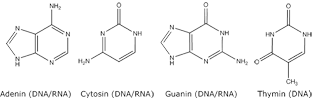
\includegraphics[scale=4]{dnabaserne.png}
\end{center}
\caption{The four different nucleobases found in the DNA nucleotides.\cite{DNA-biotechacademy}}
\end{figure}

The order of these nucleobases is what decides what function is encoded in any specific strand of DNA. A sequence of these nucleobases (a DNA sequence) is a sort of a genetic blueprint for proteins. During the production of proteins, a DNA sequence is either copied, or transcribed into ribonucleic acid (RNA), which decides which amino acids will be put together, which creates a corresponding protein.

RNA differentiates itself from DNA, among other things, by using uracil (U) instead of thymine. However, uracil and thymine is generally considered synonymous, as both bases binds with adenine.

A DNA strand can bond with another DNA strand containing the complementary nucleobases.

\begin{definition}
\textbf{complementarity} is defined as a nucleobase capable of bonding with another nucleobase.
\begin{center}
\begin{tabular}{|c|c|}
\hline
Base & Complementary base \\
\hline
G & C \\
T/U & A \\
C & G \\
A & T/U \\
\hline
\end{tabular}
\end{center}
\end{definition}

\begin{figure}[H]
	\label{Complementarity}
	\begin{center}
		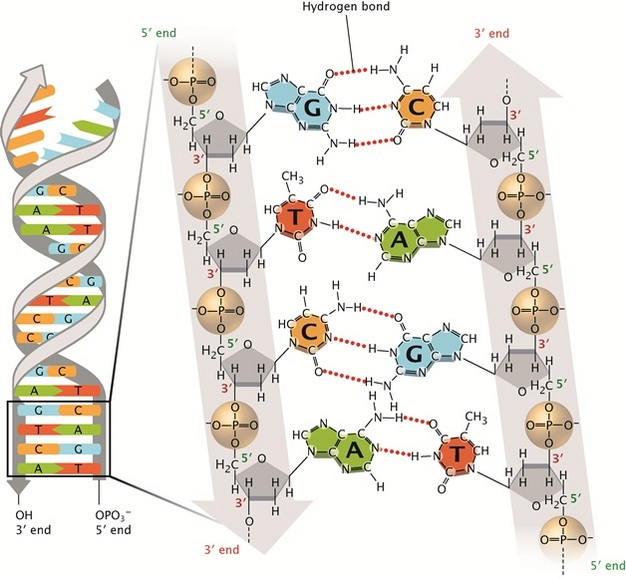
\includegraphics[scale=2.5]{complementarity.jpg}	
	\end{center}
	\caption{This figure shows the hydrogen bonds between the nucleobases, which makes up the basis for complementarity.\cite{DNA-nature}}
\end{figure}

Sometimes, you may wish to express a DNA sequence's complementary DNA sequence. This is called the complement of a given DNA sequence. The reverse of a complement is called the \textbf{reverse complement}.

\begin{definition}
For a given DNA sequence s, \~{s} is the sequence that contains the complementary bases of s, in reverse order.
\end{definition}

\subsection{Regular Expressions (TODO)}

In order to talk about regular expressions, we need to be able to talk in general terms of languages. We can define a language as a subset of the infinite set of words or symbols, chosen from a finite alphabet. An alphabet with the letters $\{a,b\}$ might for an example form the words $ab$, $ba$, $aab$ or any such conbination of any length, thus forming an infinite set of words.\\

\begin{definition} An alphabet $\Sigma$ is defined as a finite set of characters.

\end{definition}

\begin{definition} Given an alphabet $\Sigma$, the language $\mathcal{L}$ is defined by $\mathcal{L} \in \Sigma^*$, where $\Sigma^*$ is the set of all words constructed from alphabet $\Sigma$.
	
\end{definition} 

\begin{definition} Given an alphabet $\Sigma$ consisting of a finite set of characters, we can define a regular expression $E$.\\

	\begin{enumerate}
		\item An expression containing a single letter $a$ from our alphabet $\Sigma$: $E = a$. 
		\item The expression which always matches $E = 1$
		\item The expressions which never matches $E = 0$.
		\item A combination of the two regular expressions $E_1$ and $E_2$:
		\begin{eqnarray}
			E &=& E_1 | E_2 \\
			E &=& E_1E_2 \\
			E &=& E_1^*
		\end{eqnarray}
	\end{enumerate}	
\end{definition} 

\newpage

We can interpret the regular expression $E$ over the alphabet $\Sigma$ as a language denoted by $\mathcal{L}(E)$: \\

\begin{definition} The language $\mathcal{L}(E)$ for the regular expression $E$ from the alphabet $\Sigma$, can be defined as.

	\begin{enumerate}
		\item For single-letter expressions we have
			\begin{eqnarray}
				\mathcal{L}(0) &=& \emptyset \\
				\mathcal{L}(1) &=& \epsilon \\
				\mathcal{L}(a) &=& \{a\}
			\end{eqnarray}
			Where $a \in \Sigma$
			
		\item For combined expressions we have
			\begin{eqnarray}
				\mathcal{L}(E_1|E_2) &=& \mathcal{L}(E_1) \cup \mathcal{L}(E_2) \\
				\mathcal{L}(E_1E_2) &=& \mathcal{L}(E_1) \odot \mathcal{L}(E_2) \\
				\mathcal{L}(E^*) &=& \bigcup^{\infty}_{n = 0}\mathcal{L}(E^n)
			\end{eqnarray}
			Where $\mathcal{L}(E_1) \odot \mathcal{L}(E_2) = \{w_1w_2 \ |\  w_1 \in \mathcal{L}(E_1), w_2 \in \mathcal{L}(E_2)\}$, and where \\
			$E^0 = 1, \ E^{n+1} = EE^n$.
	\end{enumerate}
\end{definition}


\subsubsection{Implementing regular expressions}

Now that we have defined regular expressions formally, we want to be able to match them against strings. We say that a regular expression $E$ match a string $S$ if $S \in \mathcal{L}(E)$.
The most common way of solving this problem, and also the way industry standard regular expression implementations such as google's RE2 solve this problem\cite{matching-in-the-wild}, is through expressing the regular expression as a \textit{finite automaton}.\\

\begin{definition} A \textbf{finite automaton} can be defined as a five tuple $(Q, \Sigma, \delta, q_0, F)$ where
\label{finite automaton defintion}

\begin{itemize}
	\item $Q$ is the finite set of states
	\item $\Sigma$ is the language
	\item $\delta$ is the transition function $\delta \subseteq Q \times \Sigma \cup {\epsilon} \rightarrow Q$ defining any transition $(q_i \longrightarrow q_j) \in \delta$.
	\item $q_0$ is the initial state $q_0 \in Q$.
	\item $F$ is the set of accepting states $F \subseteq Q$.
\end{itemize}

\end{definition}

\ \\

For the purpose of representing regular expressions we use two types of finite automata called \textit{deterministic finite automata} or DFA and \textit{non-deterministic finite automata} or NFA.
DFA varies only slightly from definition \ref{finite automaton defintion}, in the sense that any transition from a uniqe state $q_i$ in a DFA only has one possible receiving state $q_j$.

\newpage

\section{Methods}
\subsection{PatScan as regular expressions}

The most notable of the patscan format's features, is the possibility to search for mismatches, insertions and deletions in a given sequence or stored sequence. The sequence \texttt{AGTCT} can be extended to \texttt{AGTCT[1,1,1]} in order to match up to one mismatch, up to one insertion, up to one deletion or any combination thereof. \\
This means that a sequence of length $n$ with a single mismatch will yield $n^1+1$ possible matches. \texttt{AGTCT[1,0,0]} will for instance match any of the following, where \_ represents a mismatch.

\texttt{AGTCT, \_GTCT, A\_TCT, AG\_CT, AGT\_T, AGTC\_}

If we extrapolate into $m$ mismatches, $d$ deletions, and $i$ insertions, we quickly find ourselves with approximately $n^{m^{d^{i}}}+1$ possible matches since all of our mismatches can be combined with all of our deletions, which in turn can be combined with all of our insertions. This is not something easily replicated with regular expressions, as we shall see in the following sections.

Another powerful feature of patscan is the ability to store a sub-pattern match in a named variable. If a match is found for the named variable in the beginning of a pattern for instance, this match can then be referenced later in the same pattern, by using the variable name. \\
An example of this could be the pattern \texttt{p1=2...4 10...20 {\raise.17ex\hbox{$\scriptstyle\mathtt{\sim}$}}p1}. This pattern will match the contents of \texttt{p1}, followed by any 10 to 20 characters, followed by the match stored in \texttt{p1}, but with the reverse complement as denoted by the \texttt{{\raise.17ex\hbox{$\scriptstyle\mathtt{\sim}$}}}.\\
This is similar to the back-referencing functionality for capturing groups, which many popular regular expression implementations support.%\cite{indsæt citation her.}

Combining this combination notation with the ability to store sequences in variables and matching them further down the pattern, makes the patscan language very compact compared to regular expressions. \\
A pattern as simple as \texttt{p1=8...16 10...50 ~p1[2,0,1]} describes a complex relationship, which cannot easily be discovered through REs.

\subsubsection{Grammar}
\label{Patscan grammar}
Scan-for-patches has an alphabet, which is the set of characters allowed in a patscan sequence. This set is from the nucleobases, that is found in DNA and RNA.
\begin{definition}
The alphabet, that makes up DNA sequences, denoted by $\mathcal{A}_{DNA}$ is:
\begin{center}
$\mathcal{A}_{DNA}$ = \texttt{\{A, T, C, G\}}
\end{center}
\end{definition}

\begin{definition}
The alphabet, that makes up RNA sequences, denoted by $\mathcal{A}_{RNA}$ is:
\begin{center}
$\mathcal{A}_{RNA}$ = \texttt{\{A, U, C, G\}}
\end{center}
\end{definition}

Besides the five basic nucleobases in $\mathcal{A}_{DNA} \cup \mathcal{A}_{RNA}$, 11 ambiguity characters also exist.\cite{DNA-sciencedaily} These ambiguity characters were designed for positional variations in families of related genes. The ambiguity characters are named so because they represent  an uncertainty of which nucleobases is actually at that spot.

\begin{definition}
The alphabet, that makes up DNA and RNA sequences, as well as the ambiguity characters, denoted by $\mathcal{A}$ is:
\begin{center}
$\mathcal{A}$ = \texttt{\{A, T, U, G, C, Y, R, S, W, K, M, B, D, H, V, N\}}
\end{center}
\end{definition}

The patscan language has the following grammar, and char is any character from the alphabet $\mathcal{A}$.

\begin{figure}[H]
\begin{center}
\begin{tabular}{|lcll|}
	\hline
	$Prog$ & $\rightarrow$ & $StmtSeq$ & \\
	$StmtSeq$ & $\rightarrow$ & list of $Stmt$ & \\
	$Stmt$ & $\rightarrow$ & $Exp$ & \\
	\enspace & $|$ & $LVal1\ =\ Exp$ &  \textcolor{red}{Variable assignment} \\
	\enspace & $|$ & $LVal2$ & \textcolor{red}{Variable usage} \\
	$LVal1$ & $\rightarrow$ & \textbf{Id} & \textcolor{red}{Ids may not be reassigned}\\
	$LVal2$ & $\rightarrow$ & \textbf{Id} $Combi$ & \\
	\enspace & $|$ & {\raise.17ex\hbox{$\scriptstyle\mathtt{\sim}$}} \textbf{Id} $Combi$ & \\
	$Exp$ & $\rightarrow$ & \textbf{num} ... \textbf{num} & \textcolor{red}{Range} \\
	\enspace & $|$ & $Seq\ Combi$ & \\
	$Seq$ & $\rightarrow$ & list of \textbf{char} & \\
	$Combi$ & $\rightarrow$ & [\textbf{num},\textbf{num},\textbf{num}] & \\
	\enspace & $|$ & $\epsilon$ & \\
	\hline
\end{tabular}
\end{center}
\caption{PatScan grammar}
\end{figure}

The patscan language can be broken down into a few simple components or tokens, which we will refer to as sub-patterns. We have divided the sub-patterns into the following classes:

\begin{definition}
The sub-patterns, that consists only of a consecutive sequence of characters from $\mathcal{A}$, is denoted as a \textbf{sequence} (Example: \texttt{AGTCT})
\\\\
The sub-patterns, that consists of a consecutive sequence of characters from $\mathcal{A}$, followed by square brackets, containing three numbers (each representing \textbf{mismatches}, \textbf{deletions}, and \textbf{insertions} respectively), is denoted as a \textbf{combination sequence} (Example: \texttt{AGTCT[1,0,0]})
\\\\
The sub-patterns, that consists of a number, $a \geq 0$, followed by exactly three dots, followed by a number, $b \geq a$, is denoted as a \textbf{range} (Example: \texttt{2...4})
\\\\
The sub-patterns, that consists of a string, denoted as a \textbf{variable name}, followed by an equal sign, and then a \textbf{sequence}, is denoted as a \textbf{variable assignment} (Example: \texttt{p1=AGTCT})
\\\\
The sub-patterns, that consists only of a \textbf{variable name}, is denoted as a \textbf{variable usage} (Example: \texttt{p1})
\\\\
The reverse complement of a sequence or variable is denoted by placing a \texttt{{\raise.17ex\hbox{$\scriptstyle\mathtt{\sim}$}}q1} directly in front of the sequence or variable.
\end{definition}

\subsubsection{Ranges}

Patscan ranges are very similar to RE ranges, and is therefore easily translated. A patscan range, which has the following form:
\begin{equation}
\label{example:range}
	2...5
\end{equation}
It translates into 'between 2 and 5 of any character'. In RE, there is a character for 'any character', which is \texttt{.}, and a quantifier, where you can state how many of a given character you want matched, which is \texttt{\{min,max\}}. Using these, (\ref{example:range}) translates into the following RE:
\begin{equation}
.\{2,5\}
\end{equation}

\subsubsection{Mismatches, Deletions, and Insertions}

Combination sequence sub-patterns can have the following form, which allows for mismatches, deletions and insertions in the sub-pattern. 
\begin{equation}
	Sequence[m, d, i] \ \ \{m, d, i \in \mathbb{N}_0 \}
\end{equation} 

This notation allows for up to the given number of mismatches, deletions or insertions. This means we for example can have $m$ mismatches and $i$ insertions, but not necessarily $d$ deletions.

This kind of notation does not exist in REs. One way to represent these sub-patterns as REs is by constructing every possible combination of the sequence, matching the patscan notation, which is the problem we sought to solve.

Recursion can be used to solve this problem. However, using recursion alone comes with some problems, that we had to address. 

A simple way to find all possible combinations is by looking at each letter in the sequence, and run the algorithm for each possibility for that letter

\begin{example}[label=example:recursion]
Looking at the combination sequence \texttt{AGCTC[2,0,0]}, we start by taking the \texttt{A}, and run the algorithm with the remaining letters for every possibility of the \texttt{A}.
\begin{eqnarray}
	Left\ branch &=& func(\texttt{A}, \texttt{GCTC[2,0,0]}) \\
	right\ branch &=& func(mismatch(\texttt{A}), \texttt{GCTC[1,0,0]})
\end{eqnarray}
The left branch will continue recursively with \texttt{GCTC[2,0,0]}, and the right branch will do the same but with only one mismatch available, since we already chose \texttt{A} as our first mismatch. When no more recursion steps can be taken, we will have a string with a unique combination of mismatches.Like this, all possible combinations will be constructed, and they can be added to a list of all combinations. Like this, all possible combinations will be constructed.
\end{example}

Adding deletions and insertions to \textbf{example \ref{example:recursion}} will increase the number of possibilities for each letter, thus increasing the amount of recursion. The recursion does not stop until every combination is found, which means that if the sequence is large enough (This can happen already at a length of 20, if not earlier, depending on the number of mismatches, insertions, and deletions), the program can reach maximum recursion depth (depending on the programming language), or run out of memory before terminating.

In order to guarantee a low recursion depth, we use a divide and conquer algorithm\cite{Algorithms} instead, that reduces the recursion depth to $log(n)$. This works by splitting the sequence in two halves per recursion, such that at the deepest recursion level, we have a single sequence of only a single character, as can be seen in figure \ref{fig:tree_example}. 

\begin{figure}[H]
\begin{tikzpicture}[->,>=stealth',level/.style={sibling distance = 5cm/#1,
  level distance = 1.5cm}] 
\node [arn_n] {abcd}
	child{ node [arn_n] {ab} 
		child{ node [arn_n] {a}}
		child{ node [arn_n] {b}}                            
	}
    child{ node [arn_n] {cd}
		child{ node [arn_n] {c}}
		child{ node [arn_n] {d}}
	}
; 
\end{tikzpicture}
	\centering
	\caption{Tree structure, showing the steps taken by the algorithm during the divide step.}
	\label{fig:tree_example}
\end{figure}

After dividing the sequence into characters, we have to 'conquer' each sub-problem. On the lowest recursion level (where the sequence is a single character), the algorithm will make a list of all possibilities, which that character can be.

\begin{example}[label=example:possibilities]
For character 'a' from figure \ref{fig:tree_example}, we have the following possibilities for mismatches and deletions

\begin{center}
	{a, \^{}a, \_}
\end{center}

as well as the following for insertions

\begin{center}
	\texttt{.\{1\}a, .\{2\}a, $\cdots$, .\{n\}a} \\
	\texttt{a.\{1\}, a.\{2\}, $\cdots$, a.\{n\}}
\end{center}

A list of all these possibilities is then returned, and it can be combined with the list received from the 'b' recursion.
\end{example}

These lists are combined by taking each outcome from the first list, and combining it with each outcome of the second list. The total number of mismatches, deletions, and insertions are being kept track of, and if combining two outcomes will result in more mismatches, deletions, or insertions than the maximum allowed, it is skipped.

\begin{spacing}{0.8}
\begin{algorithm}[H]
	\caption{find\_combinations (Divide and conquer)}
	\label{alg:divideandconquer}
  	\begin{algorithmic}[1]
    		\Require
    			\Statex $seq$ - sequence string to be translated
    			\Statex $m_{max}$ - allowed number of mismatches
    			\Statex $d_{max}$ - allowed number of deletions
    			\Statex $i_{max}$ - allowed number of insertions
    		\Ensure
    			\Statex List of all possible combinations
		\Statex
		\Function{find\_combinations}{$seq$, $m_{max}$, $d_{max}$, $i_{max}$}
    		\If{$seq.length > 1$}
    			\Let{left\_tree}{\Call{find\_combinations}{seq[0..(seq.length/2).floor-1], $m_{max}$, $i_{max}$, $d_{max}$}}
    			\Let{right\_tree}{\Call{find\_combinations}{seq[(seq.length/2).floor..-1], $m_{max}$, $i_{max}$, $d_{max}$}}
    		\Else
    			\Returns{List of all mismatch, insertion, and deletion combinations of seq}
    		\EndIf
    		\State
    		\Let{combined}{empty list}
    		\Let{unique\_combinations}{empty set}
    		\ForAll{LL \In left\_tree} \Comment{LL: Left leaf}
    			\ForAll{RL \textbf{in} right\_tree} \Comment{RL: Right leaf}
    				\If{$LL.m + RL.m > m_{max}$ \Or $LL.d + RL.d > d_{max}$ \Or $LL.i + RL.i > i_{max}$}
    					\State continue
    				\EndIf
    				\If{\Not LL.seq + RL.seq \In unique\_combinations.keys}
    					\Append{unique\_combinations}{LL.seq + RL.seq}
    					\Append{combined}{LL + RL}
    				\EndIf
    			\EndFor
    		\EndFor
    		\Returns{combined}
    		\EndFunction
  	\end{algorithmic}
\end{algorithm}
\end{spacing}

\subsubsubsection{Redundancy}

Using algorithm \ref{alg:divideandconquer} without modifications, we will have a lot of redundancy when translating insertions. This comes from the fact, that we wish to construct all possible combinations, and that we do it recursively.

If we look at the combination sequence \texttt{ab[0,0,1]}, the possible outcomes of \texttt{a} (at the lowest level of recursion) can be \texttt{a}, \texttt{.a}, and \texttt{a.}, and the same for \texttt{b}. Combining these, we will have two different cases of \texttt{a.b} (\texttt{a. b} and \texttt{a .b}). It is redundant to keep both, and by keeping it, will create exponentially more redundancy, the more levels of the recursion there is.

Assuming we have an even number of characters in the sequence, and that only insertions are allowed, we have that on the first 'combine' step, there is $r_0$ redundant cases. In the following example, $i_{max}$ is the maximum number of allowed insertions.

\begin{example}
The following example shows the variations of a with b that are the same when combined. The bold characters are combined with the cursive characters.
\begin{eqnarray}
	i_{1}: \textbf{a.}b\ \ \textbf{a}.b = 2 - 1 = 1 \\
	i_{2}: \textbf{a..}b\ \ \textbf{a.}.b\ \ \textbf{a}..b = 3 - 1 = 2 \\
	i_{3}: \textbf{a...}b\ \ \textbf{a..}.b\ \ \textbf{a.}..b\ \ \textbf{a}...b = 4 - 1 = 3
\end{eqnarray}
Here, for $i_{1}$, we have 2 cases, that are the same. One of those are redundant, thus $2 - 1 = 1$ redundant case. \\
Since all cases for $i_{n-1}$ also applies to $i_{n}$, we end up with
\begin{eqnarray}
	\sum_{i=1}^{i_{max}}i
\end{eqnarray}
redundant cases for each combination step in each branch. If $n$ is the number of characters in the sequence, there are $\frac{1}{2}n$ combination steps on this level, which gives us:
\begin{eqnarray}
	\label{r_0}
	r_0 = \frac{1}{2}n\sum^{i_{max}}_{i=1} i
\end{eqnarray}
\end{example}

On the next combine step, we have $r_1$ redundant cases. In order to calculate $r_1$, I will define $c = 1 + 2i$ as the number of cases in the \textit{base case}, meaning the number of cases in the lowest level of recursion. Each redundant case will be combined with all cases in the second set, which contains $c^2$ cases. All non-redundant cases from the first set will also be combined with all redundant cases of the second set. Because there is maximum of the number of insertions allowed in a single case, where this maximum varies, we will introduce a factor $\kappa$, that represents the scaling factor, that corrects the number of elements in a given set, corresponding to the number of insertions allowed.
\begin{eqnarray}
	2r_0\frac{c^2}{\kappa_0} - r_0^2
\end{eqnarray}

\begin{example}
We have a set $A$ and another set $B$, each containing $\frac{c^2}{\kappa}$ elements, of which $r_0$ are redundant.

All $r_0$ redundant elements in $A$ will combine with all elements in $B$, creating $r_0\frac{c^2}{\kappa}$ redundant cases. Likewise, all $\frac{c^2}{\kappa}-r_0$ non-redundant case in $A$ will combine with all $r_0$ redundant cases in $B$, creating $r_0(\frac{c^2}{\kappa}-r_0)$ additional redundant cases. There are $\frac{1}{4}n$ combination steps on this level, which gives us:
\begin{eqnarray}
	\label{r_1}
	r_1 &=& \frac{1}{4}n(r_0\frac{c^2}{\kappa_1} + r_0(\frac{c^2}{\kappa_1} - r_0))\\
		&=& \frac{1}{4}n(r_0\frac{c^2}{\kappa_1} + r_0\frac{c^2}{\kappa_1} - r_0^2))\\
		&=& \frac{1}{4}n(2r_0\frac{c^2}{\kappa_1} - r_0^2)
\end{eqnarray}
\end{example}

We can then calculate the total amount of redundancy of any sequence with $logn$ recursion depth, via induction:
\begin{eqnarray}
	r_x &=& \frac{1}{2^{x+1}}n (r_{x-1}\frac{c^{2^{x+1}}}{\kappa_x} + r_{x-1}(\frac{c^{2^{x+1}}}{\kappa_x} - r_{x-1}))\\
		&=& \frac{1}{2^{x+1}}n (r_{x-1}\frac{c^{2^{x+1}}}{\kappa_x} + r_{x-1}\frac{c^{2^{x+1}}}{\kappa_x} - r_{x-1}^2)\\
		\label{r_x}
		&=& \frac{1}{2^{x+1}}n (2r_{x-1}\frac{c^{2^{x+1}}}{\kappa_x} - r_{x-1}^{2^{x+1}})
\end{eqnarray}

Here, $x$ is the recursion depth, and will thus go up to $logn$, where $n$ is the length of the patscan sequence.

Given a pattern, where mismatches and deletions are allowed as well as insertions, the amount of redundancy increases, as $c$ will become larger.

Despite result reached in formula \ref{r_x}, inaccuracy occurs, as the recursion depth varies in the recursion branches based on the length of the original string, like in figure \ref{fig:recursion_depth_example}.

\begin{figure}[H]
\begin{tikzpicture}[->,>=stealth',level/.style={sibling distance = 5cm/#1,
  level distance = 1.5cm}] 
\node [arn_n] {abc}
	child{ node [arn_n] {a}}
    child{ node [arn_n] {bc}
		child{ node [arn_n] {b}}
		child{ node [arn_n] {c}}
	}
; 
\end{tikzpicture}
	\centering
	\caption{Tree structure showing how recursion depth varies in different branches.}
	\label{fig:recursion_depth_example}
\end{figure}

Despite of this inaccuracy, it is still trivial, that the amount of redundancy in is excessive, as it translates directly into additional running time.

Avoiding this redundancy is very important, and relatively trivial. Every time two cases are combined, it is used as a key in a hash table, and its value set to true. The value doesn't matter, all that matters is that the hash table now has this combination as a key.

Every time we make a new combination, we check if that combination already exists, and if it does, we simply skip it.

We can look up in a hash table in $O(1)$ time, which doesn't increase the running time by much. However, we will end up with a significantly lower running time in the long run, as all redundancy is sorted out.

\subsubsection{Variable assignments \& usage}

Variable assignment is when you have a pattern of some sort, that you assign to a variable, so that it may be reused later. Any kind of non-variable pattern may be used in a variable pattern. Hence, we have three different variable assignments:

\texttt{p1=ATCG} \\
\texttt{p2=ATCG[2,0,0]} \\
\texttt{p3=2...4}

These assignments can be referenced by using the variable name. An example of such usage could be

\texttt{q1=ACCT 2...5 q1}

In addition to referencing the variable, a variable may also be inverted. This is denoted by using a tilde character prepended to the variable:

\texttt{{\raise.17ex\hbox{$\scriptstyle\mathtt{\sim}$}}q1}

Here, inversion refers to the reverse complement of the sequence stored in the variable.

Sequence and combination assignments are implemented by translating the sequence/combination and storing the translated regular expression in a table, with the variable name as the key. Then, if the variable is used later in the patscan pattern, the translated sequence/combination may be placed into the full regular expression. This way, there are no actual referencing in the regular expression, keeping the expressions regular.

Assignment of a range is something we have chosen not to implement, as it can't be implemented without the use of back-referencing. This is because there's no way of knowing what a range will actually be besides x-y random characters. Because of this inherent ability to change, depending on where in the file the engine is matching, it is not possible to 'hard code' it as a regular expression.

Using back-referencing in our implementation will cause our RE patterns to lose regularity, and with that, performance.

\subsection{Correctness}

Pre-conditions:\\
seq is a string of length $i > 0$\\
$m_{max}$ is a non-negative integer\\
$d_{max}$ is a non-negative integer\\
$i_{max}$ is a non-negative integer

post-condition:\\
\textbf{combined} contains all combinations of the initial sequence with up to  $m_{max}$ mismatches, $d_{max}$ deletions, and $i_{max}$ insertions.

\textbf{Recursion:}

For merging in algorithm \ref{alg:divideandconquer}, we have the invariant I(n): \textbf{For a set $A$, and a set $B$, a combination of the two, where each element in $A$ is combined with each element in $B$ separately, yields a set $C$, such that all $e \in C$ satisfies $e_m \leq m_{max}$, $e_d \leq d_{max}$, $e_i \leq i_{max}$}

\begin{itemize}
\item Initialization:
\begin{itemize}
	\item[] Prior to the merging step, the invariant is respected (trivially), as set $A$ and $B$ is empty.
\end{itemize}

\item Maintenance:
\begin{itemize}
	\item[] For merging step $k$, the algorithm will have two sets of valid elements (respects the condition in the invariant), from which it will construct a new set of all combinations of the elements in the two original sets. Any combination that would not satisfy the condition will never be created in the first place.
\end{itemize}

\item Termination:
\begin{itemize}
	\item[] When the recursion terminates, the invariant will be true on the entire output.
\end{itemize}
\end{itemize}

\textbf{Outer loop:}

For the outer loop we have the following invariant: \textbf{For an element $A[i]$, combining it with each element in a set $B$, yields a new set $C$, such that all $e \in C$ satisfies $e_m \leq m_{max}$, $e_d \leq d_{max}$, $e_i \leq i_{max}$}

\begin{itemize}
\item Initialization:
\begin{itemize}
	\item[] For $i = 0$, the invariant is respected (trivially), as $A[i]$ and $B$ are empty.
\end{itemize}

\item Maintenance:
\begin{itemize}
	\item[] For $i = k$, the loop will have an element $A[i]$, and a set of valid elements (respects the condition in the invariant), from which it will construct a new set of all combinations of $A[i]$, and the set $B$. Any combination that would not satisfy the condition will never be created in the first place.
\end{itemize}

\item Termination:
\begin{itemize}
	\item[] When the loop terminates, the invariant will be true on the entire output.
\end{itemize}
\end{itemize}

\textbf{Inner loop:}

For the inner loop we have the following invariant: \textbf{For an element $a$, and another element $B[j]$, a combination of the two yields a new element $c$, such that it satisfies $c_m \leq m_{max}$, $c_d \leq d_{max}$, $c_i \leq i_{max}$}

\begin{itemize}
\item Initialization:
\begin{itemize}
	\item[] For $j = 0$, the invariant is respected (trivially), as $a$ and $B[j]$ are \textbf{null}.
\end{itemize}

\item Maintenance:
\begin{itemize}
	\item[] For $j = k$, the loop will have an element $a$, and an element $B[j]$, which both respect the condition in the invariant. $a$ and $B[j]$ will be combined to a new element $c$. If the condition in the invariant is not satisfied, construction of $c$ will be skipped, maintaining a true invariant.
\end{itemize}

\item Termination:
\begin{itemize}
	\item[] When the loop terminates, the invariant will be true on the output.
\end{itemize}
\end{itemize}

\subsection{Running time}

In the divide step, our algorithm (algorithm \ref{alg:divideandconquer}) first splits a given sequence in half multiple times until it reaches base case (where length of the sequence is one). It does this recursively with a branching factor of two, meaning the running time so far is 
\begin{eqnarray}
	T(n) = 2T(\frac{n}{2}) = O(log_2n)
\end{eqnarray}

The conquer step, where we construct each combination of every base case, is trivially solved by constructing a set of the combinations. It constructs one element if any mismatches are allowed, which it can do in $O(1)$ constant time. It constructs one element if any deletions are allowed, which it can also do in $O(1)$ constant time. It constructs two elements for each insertions that is allowed, which take $O(2i)$ time. It does this for every base case, which leaves us with a total running time of $O(ni)$, where $i$ is the number of insertions allowed.
\begin{eqnarray}
	T(n) = O(log_2n) + O(ni)
\end{eqnarray}

In the combine step, we combine each element of two sets $A$ and $B$. Each combination takes $O(1)$ constant time, and it does this operation $SIZE(A) \cdot SIZE(B)$ times. The sets $A$ and $B$ were created in the same way recursively, which means the total running time of each recursion level increases exponentially. In total we have a running time of $O(i^{2^{log_2(n)}})$, where $i$ is the number of insertions, and $n$ is the length of the sequence.

The running time of every combination step before the final one combined is significantly smaller than the final combination step, which means that they are consumed by the exponentially larger running time of the last iteration. This gives us a running time of:
\begin{eqnarray}
	T(n) = O(log_2n) + O(ni) + O(i^{2^{log_2(n)}})
\end{eqnarray}

The running time of the divide and conquer step also consumed by the combine step, leaving us with a running time of
\begin{eqnarray}
	O(i^{2^{log_2(n)}})
\end{eqnarray}

\begin{example}
If we have the sequence \texttt{ATGCAATT[0,0,2]}, we will have a recursion depth, and thus the divide step has a running time of:
\begin{eqnarray}
	log_2(8) = 3
\end{eqnarray}

The conquer step will then have a running time of
\begin{eqnarray}
	8\cdot 2 = 16
\end{eqnarray}

The final step of the combine step will have a running time of
\begin{eqnarray}
	2^{2^{log_2(8)}} = 256
\end{eqnarray}

It can thus be seen, that the running time of the combine step consumes the running time of both the divide and the conquer step.
\end{example}


\subsection{Data Analysis (TO BE WRITTEN)}

\section{Results (TO BE WRITTEN)}

\subsection{Experiment design (TO BE WRITTEN)}

\subsection{Experiment results (TO BE WRITTEN)}

\section{Conclusion (TO BE WRITTEN)}

\newpage

\pagenumbering{gobble}
\bibliographystyle{plain}
\nocite{*}
\bibliography{litterature}

\end{document}
